\documentclass[xcolor=dvipsnames,12pt]{beamer} %pt10,11,12
\usefonttheme{serif}
\usepackage{graphicx}
%%\usepackage{subfigure}
\usepackage{multicol}
\usepackage[figurename=]{caption}
%%\usepackage{xcolor}
\usepackage{hyperref}
\hypersetup{
    colorlinks=true,%
    citecolor=blue,%
    filecolor=black,%
    linkcolor=blue,%
    urlcolor=blue
}


\setlength{\parskip}{2ex}

\title{Using Latent Variable Models to Estimate the Prevalence of Sexual Violence in Armed Conflict: An Introduction}
\author{Jule Kr\"{u}ger, \\ Center for Political Studies, University of Michigan\\[.5cm]
\emph{Workshop on Empirical and Computational Social Sciences in India}\\[.5cm] Ashoka University, December 15, 2018}
\date{}
\begin{document}

\frame{\titlepage}

\frame{
This workshop builds on ongoing research with

\begin{multicols}{2}

\begin{figure}
\includegraphics[width=4cm]{hand/RNordaas.jpeg}\caption{\href{https://ragnhildnordas.wordpress.com/}{Ragnhild Nord\r{a}s}}
\end{figure}
and 
\begin{figure}
\includegraphics[width=5cm]{hand/CFariss.jpg}\caption{\href{http://cfariss.com/}{Christopher Fariss}}
\end{figure}
\end{multicols}

}

\frame{\frametitle{Wartime Sexual Violence}

\begin{itemize}
\item Includes the use of rape and other forms of sexual violence
\item Constitutes a severe human rights problem
\item Is difficult to observe and document as a practice
\end{itemize}

A lack of systematic data impedes empirical analysis with regard to extent, spatiotemporal trends, and patterns.

}

\frame{\frametitle{Why Conflict-Related Sexual Violence  Is Hard to Measure}
\begin{itemize}
\item Shame, fear of retaliation, stigma and rejection due to socio-cultural taboos
\item Inconsistency in testimony and lack of clear narrative due to trauma-induced memory loss
\item Differing conceptualizations and language  used to refer to sexual violence events
\item Perpetrators' incentives to conceal activity and evade accountability for war crimes
\item Blending of state actors and institutions with regard to the perpetration and reporting of these crimes

\end{itemize}

All of these issues vary over space and time.

}

\frame{\frametitle{Why the Observation of Wartime Sexual Violence May Improve over Time}

\begin{itemize}
\item Increasing international focus
\item Changing norms and perceptions of survivors
\item Recent challenges to societal taboos
\item Growing initiatives to empower survivors to speak out
\item Changes in the wording of sexual violence experiences leading to more explicit descriptions
\item Growth in documentation efforts paired with improved documentation practices
\end{itemize}

While these trends  vary across space, we will likely see higher reporting rates in some places  over time.

}

\frame{\frametitle{How We Currently Measure Wartime Sexual Violence}

\begin{figure}
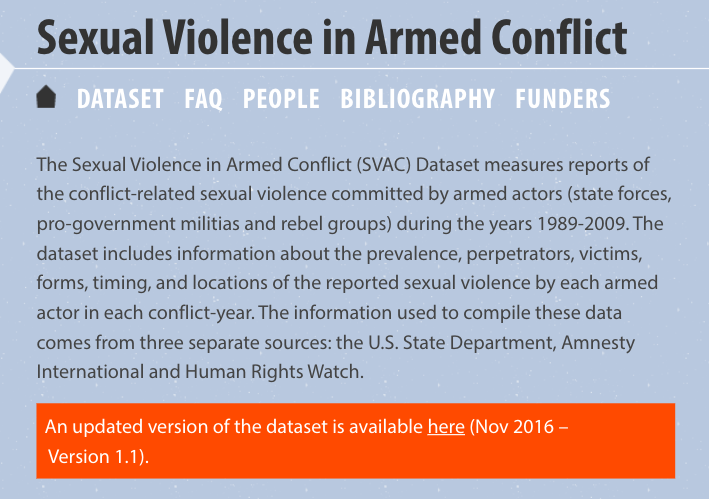
\includegraphics[width=9cm]{hand/SVAC-home.png}
\caption{SVAC, \url{http://www.sexualviolencedata.org/}}
\end{figure}
}

\frame{Let's import the data into R and take a look at it:

\begin{itemize}
\item[{\tt \$:}] {\tt cd \textasciitilde/git/SVAC-LVM-tutorial/import}\\
\item[{\tt \$:}]  {\tt open -a Rstudio src/import-check-data-main.R}
\end{itemize}

}



\begin{frame}[label=SUDAN-obs]
\frametitle{SVAC Provides Three Indicators that Report Prevalence of Wartime Sexual Violence}
\begin{figure}\centering
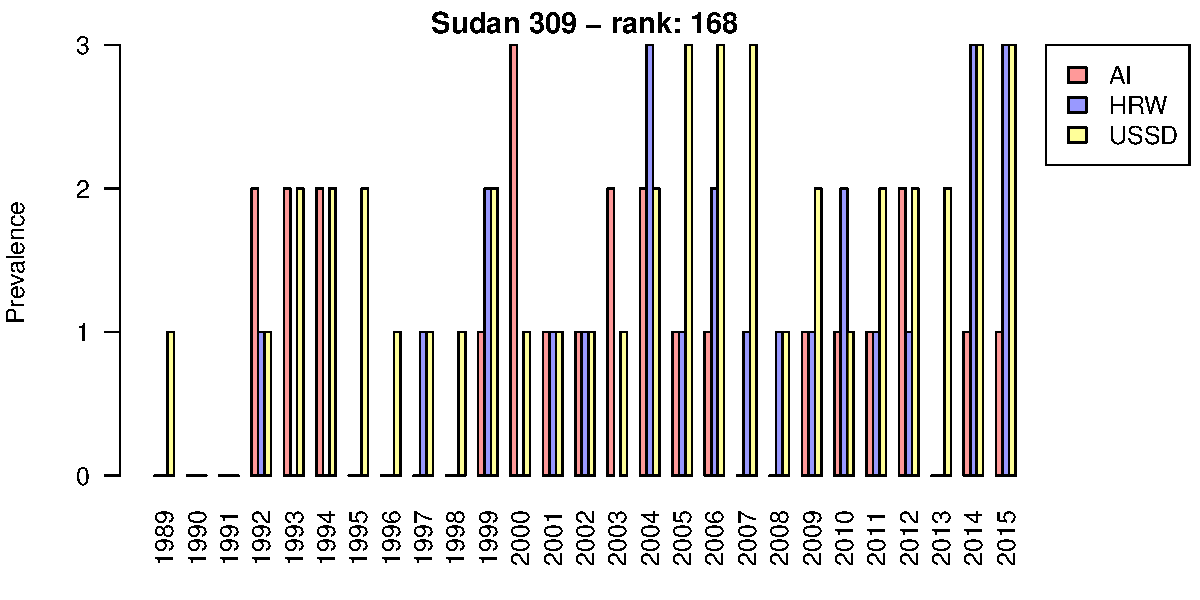
\includegraphics[width=11cm]{../visualize/output/bp-obs-GOV-Sudan-309.pdf}
\caption{Reported level of engagement in wartime sexual violence by state forces in Sudan according to three sources \hyperlink{SUDAN-est}{\beamerbutton{est}}}
\end{figure}
\end{frame}


\begin{frame}[label=DRC-obs]
\frametitle{Another Case... }
\begin{figure}\centering
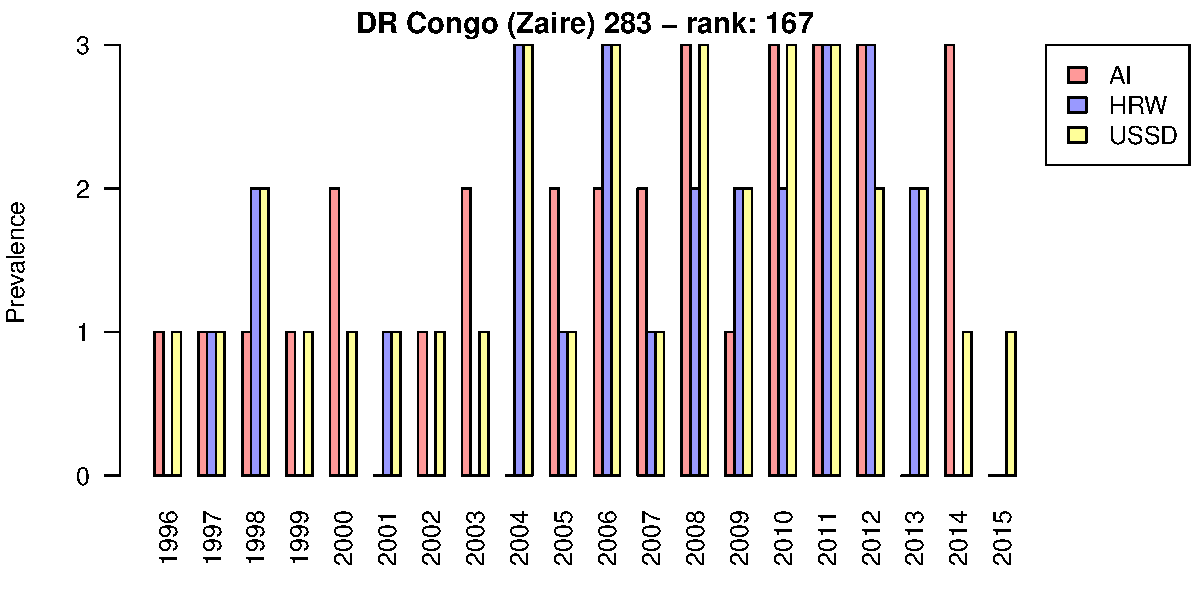
\includegraphics[width=11cm]{../visualize/output/bp-obs-GOV-DR-Congo-Zaire-283.pdf}
\caption{Reported level of engagement in wartime sexual violence by state forces in DRC according to three sources \hyperlink{DRC-est}{\beamerbutton{est}}}
\end{figure}
\end{frame}

\frame{

Let's make some more barplots of reported state behavior for other armed conflict cases:

\begin{itemize}
\item[{\tt \$:}] {\tt cd ../visualize}
\item[{\tt \$:}] {\tt open -a Rstudio  src/barplot-sources-by-conflict.R}
\end{itemize}

}

\frame{\frametitle{The Promise of Latent Variable Models for Measuring Sexual Violence}}
%% theoretical construct of interest: prevalence of sexual violence committed by GOV troups
%% assumption that there is an underlying latent trait that can be estimated using observed outcomes (items/responses/reports)
%% standard ordinal item response model: ordinal indicators
%% perceptual errors by coders and reporting error by organizations: logistic distribution of the error term
%% local independence assumption: any two item responses are independent (only related in that they measure the same latent trait) (1) within same country-year, (2) across countries within years, (3) across years within countries --> (3) is relaxed 
%% dynamic: hierarchical priors (prior beliefs) allow estimated latent prevalence of SV to depend on that conflict's value in the previous year}






\end{document}